%!TEX encoding = UTF-8 Unicode
%!TEX root = ../algos-geometriques.tex


\chapter{Points}

Dans ce chapitre, un point $P$ est défini par ses coordonnées $(P.x, P.y)$. Les fonctions sont définies par une extension de \texttt{CGPoint} dans le fichier \texttt{extension-CGPoint.swift}.


\section{Distance entre deux points}

Élementaire !


\begin{lstlisting}
extension CGPoint {
  static func distance (_ p1 : CGPoint, _ p2 : CGPoint) -> CGFloat {
    let dx = p1.x - p2.x
    let dy = p1.y - p2.y
    return sqrt (dx * dx + dy * dy)
  }
}
\end{lstlisting}




\section{Fonction \texttt{product}}

Cette fonction permet de savoir si un point $P_3$ est situé \emph{à droite} (comme dans la figure ci-dessous) ou \emph{à gauche} d'un segment $P_1P_2$. Cette fonction est fondamentale pour de nombreux calculs, comme par exemple l'intersection de deux rectangles.

\begin{center}
  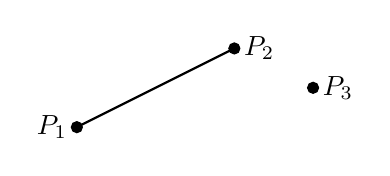
\begin{tikzpicture}
    \draw[thick] (0, 0) -- (2, 1) ;
    \draw[fill] (0, 0) circle (2pt) ;
    \draw[fill] (2, 1) circle (2pt) ;
    \draw[left] (0, 0) node {$P_1$} ;
    \draw[right] (2, 1) node {$P_2$} ;
    \draw[fill] (3, 0.5) circle (2pt) ;
    \draw[right] (3, 0.5) node {$P_3$} ;
  \end{tikzpicture}
\end{center}

Pour cela, on calcule la composante verticale du produit vectoriel $\overrightarrow{P_1P_2} \wedge \overrightarrow{P_1P_3}$ :
\begin{itemize}
\item positive, le point $P_3$ est à gauche du segment $P_1P_2$ ;
\item négative, le point $P_3$ est à droite du segment $P_1P_2$ ;
\item nulle, le point $P_3$ est aligné avec le segment $P_1P_2$.
\end{itemize}


\begin{lstlisting}
extension CGPoint {
  static func product (_ p1 : CGPoint, _ p2 : CGPoint, _ p3 : CGPoint) -> CGFloat {
    let dx2 = p2.x - p1.x
    let dy2 = p2.y - p1.y
    let dx3 = p3.x - p1.x
    let dy3 = p3.y - p1.y
    return dx2 * dy3 - dx3 * dy2
  }
}
\end{lstlisting}




\section{Angle d'un vecteur avec l'horizontal}

Étant donnés deux points $P_1$ et $P_2$, il s'agit de déterminer l'angle $\alpha$ que fait le vecteur $\overrightarrow{P_1P_2}$ avec l'horizontale :

\begin{center}
  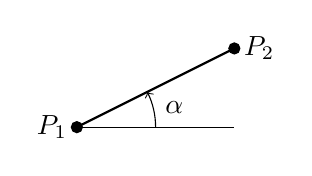
\begin{tikzpicture}
    \draw[thick] (0, 0) -- (2, 1) ;
    \draw (0, 0) -- (2, 0) ;
    \draw[fill] (0, 0) circle (2pt) ;
    \draw[fill] (2, 1) circle (2pt) ;
    \draw[left] (0, 0) node {$P_1$} ;
    \draw[right] (2, 1) node {$P_2$} ;
    \draw[->] (1,0) arc (0:26.57:1) ;
    \draw[right] (1, .25) node {$\alpha$} ;
  \end{tikzpicture}
\end{center}

La fonction \texttt{atan2} renvoie l'angle en radian, et gère tous les cas particuliers (voir le \emph{man} de cette fonction) :
\begin{itemize}
  \item \texttt{atan2(+-0, -0)} retourne $\pm\pi$ ;
  \item \texttt{atan2(+-0, +0)} retourne $\pm0$ ;
  \item \texttt{atan2(+-0, x)} retourne $\pm\pi$ pour $x < 0$ ;
  \item \texttt{atan2(+-0, x)} retourne $\pm0$ pour $x > 0$ ;
  \item \texttt{atan2(y, +-0)} retourne $+\pi/2$ pour $y > 0$ ;
  \item \texttt{atan2(y, +-0)} retourne $-\pi/2$ pour $y < 0$.
\end{itemize}



\begin{lstlisting}
extension CGPoint {
  static func angleInRadian (_ p1 : CGPoint, _ p2 : CGPoint) -> CGFloat {
    let width = p2.x - p1.x
    let height = p2.y - p1.y
    return atan2 (height, width) // Result in radian
  }
}
\end{lstlisting}
